\documentclass[]{article}
\usepackage{lmodern}
\usepackage{amssymb,amsmath}
\usepackage{ifxetex,ifluatex}
\usepackage{fixltx2e} % provides \textsubscript
\ifnum 0\ifxetex 1\fi\ifluatex 1\fi=0 % if pdftex
  \usepackage[T1]{fontenc}
  \usepackage[utf8]{inputenc}
\else % if luatex or xelatex
  \ifxetex
    \usepackage{mathspec}
  \else
    \usepackage{fontspec}
  \fi
  \defaultfontfeatures{Ligatures=TeX,Scale=MatchLowercase}
\fi
% use upquote if available, for straight quotes in verbatim environments
\IfFileExists{upquote.sty}{\usepackage{upquote}}{}
% use microtype if available
\IfFileExists{microtype.sty}{%
\usepackage{microtype}
\UseMicrotypeSet[protrusion]{basicmath} % disable protrusion for tt fonts
}{}
\usepackage[top=3cm,left=3cm,right=3cm]{geometry}
\usepackage{hyperref}
\hypersetup{unicode=true,
            pdftitle={Disease Modeling},
            pdfborder={0 0 0},
            breaklinks=true}
\urlstyle{same}  % don't use monospace font for urls
\usepackage{graphicx,grffile}
\makeatletter
\def\maxwidth{\ifdim\Gin@nat@width>\linewidth\linewidth\else\Gin@nat@width\fi}
\def\maxheight{\ifdim\Gin@nat@height>\textheight\textheight\else\Gin@nat@height\fi}
\makeatother
% Scale images if necessary, so that they will not overflow the page
% margins by default, and it is still possible to overwrite the defaults
% using explicit options in \includegraphics[width, height, ...]{}
\setkeys{Gin}{width=\maxwidth,height=\maxheight,keepaspectratio}
\IfFileExists{parskip.sty}{%
\usepackage{parskip}
}{% else
\setlength{\parindent}{0pt}
\setlength{\parskip}{6pt plus 2pt minus 1pt}
}
\setlength{\emergencystretch}{3em}  % prevent overfull lines
\providecommand{\tightlist}{%
  \setlength{\itemsep}{0pt}\setlength{\parskip}{0pt}}
\setcounter{secnumdepth}{5}
% Redefines (sub)paragraphs to behave more like sections
\ifx\paragraph\undefined\else
\let\oldparagraph\paragraph
\renewcommand{\paragraph}[1]{\oldparagraph{#1}\mbox{}}
\fi
\ifx\subparagraph\undefined\else
\let\oldsubparagraph\subparagraph
\renewcommand{\subparagraph}[1]{\oldsubparagraph{#1}\mbox{}}
\fi

%%% Use protect on footnotes to avoid problems with footnotes in titles
\let\rmarkdownfootnote\footnote%
\def\footnote{\protect\rmarkdownfootnote}

%%% Change title format to be more compact
\usepackage{titling}

% Create subtitle command for use in maketitle
\providecommand{\subtitle}[1]{
  \posttitle{
    \begin{center}\large#1\end{center}
    }
}

\setlength{\droptitle}{-2em}

  \title{Disease Modeling}
    \pretitle{\vspace{\droptitle}\centering\huge}
  \posttitle{\par}
    \author{}
    \preauthor{}\postauthor{}
    \date{}
    \predate{}\postdate{}
  
\usepackage{multirow}
\usepackage{multicol}
\usepackage{booktabs}
\usepackage{xcolor}
\numberwithin{equation}{section}
\counterwithin{figure}{section}
\counterwithin{table}{section}
\usepackage{dcolumn}
\usepackage{rotating}
\usepackage{caption}
\usepackage{amsfonts}

\begin{document}
\maketitle

{
\setcounter{tocdepth}{2}
\tableofcontents
}
\hypertarget{intro}{%
\section{Intro}\label{intro}}

Over May 2011, a strain \emph{Escherichia coli} (\emph{E. coli}) caused
an outbreak of severe illness in Germany, with \textasciitilde{}3,950
affected compared with \textasciitilde{}200 cases a year typically seen.
Of those infected 53 died.

In this - we extend a method presented by Held et al.
(\protect\hyperlink{ref-held_two-component_2006}{2006}) for modeling
parameters of infectious disease counts in a Bayesian framework. Their
method models the count data as a branching Poisson process with a
cyclical endemic parameter.

We then extend their model to incorporate a graph.

\hypertarget{comments}{%
\subsection{Comments}\label{comments}}

Expand and metion general ideas of epidemics spreading \& how we model
them (\textasciitilde{}1 page)

\hypertarget{intro-to-two-component-model}{%
\section{Intro to Two-Component
Model}\label{intro-to-two-component-model}}

Held et al. (\protect\hyperlink{ref-held_two-component_2006}{2006})
presents a stochastic model for the statistical analysis of infectious
disease counts that serves as the basis of the theextended graph model.

The two components of the model are a simple Poisson branching process
with autoregressive parameter \(\lambda\) and a seasonal component fit
with a Fourier series. These components are described as the
``epidemic'' and ``endemic'' components respectively. Additionally, the
two-component model allows for the \(\lambda\) to change over time
allowing for the disease to change infectivity over time.

\hypertarget{two-component-model-notation}{%
\subsection{Two-Component Model
Notation}\label{two-component-model-notation}}

Let \(Z = (Z_0, Z_1, ..., Z_n)\) be the infectious disease counts at
each time step \(t\). The model is then specified through
\(Z_t | Z_{t-1}\).

Each \(Z_t\) is determined as

\[ Z_t = Y_t + X_t,\ t\in\{1,\dots, n\}\]

Where \(Y_t\) is the epidemic component and \(X_t\) is the endemic
component. The epidemic component is parameterized as:
\[Y_t|Z_{t-1} \sim Pois(\lambda_tZ_{t-1})\] Where \(\lambda_t\) is
piecewise constant depending on an unknown number of changepoints \(K\)
and unknown locations \(\theta_1 < \cdots < \theta_K\).

\[ \lambda_t =  \begin{cases} \lambda^{(1)} & t < \theta_0 \\
\lambda^{(k)}, & \theta_{k} \leq t < \theta_{(k-1)} \\
\lambda^{(K+1)}, & t \geq \theta_K \end{cases}\]

The endemic component is parameterized as:

\[ X_t \sim Pois(\nu_t)\]

Where \(\log{\nu_t}\) is modeled as a Fourier series:

\[ \log{\nu_t} = \gamma_0 + \sum_{l = 1}^L \big(\gamma_{2l-1}\sin(\rho l t)+\gamma_{2l}cos(\rho l t)\big) \]

\hypertarget{epidemic-component}{%
\subsection{Epidemic Component}\label{epidemic-component}}

The epidemic component is given by:

\[Y_t|Z_{t-1} \sim Pois(\lambda_tZ_{t-1})\]

Where \(\lambda_t\) is the time varing infectivity parameter and
\(Z_{t-1}\) is the the infected count in the previous time step.

We can think of \(\lambda_t\) as the infectivity of the disease at time
\(t\) with an infected person causing new infections as
\(Pois(\lambda_t)\). Since each infected at time \(Z_{t-1}\) generates
new infected i.i.d \(Pois(\lambda_t)\), then \(Z_t\) is the sum of those
random variables which itself is Poisson;
\(\sum_1^{Z_{n-1}}Pois(\lambda_t) = Pois(\lambda_tZ_{n-1})\).

In this model, the \(\lambda_t\) is allowed to vary over time. The
parameter \(\lambda = (\lambda_1,\cdots,\lambda_n)\) is a piecewise
constant function with unknown number of changepoints \(K\) and unknown
location of changepoints \(\theta_1 < \cdots < \theta_K\) with
\(\theta \in \{1,...,n-1\}\). If \(K = 0\) there is no changepoint and
the \(\lambda\) parameter is constant throughout.

\hypertarget{tk-add-references-below}{%
\subsection{TK add references below}\label{tk-add-references-below}}

For constant \(\lambda\), this is known as a Poisson branching process.
For such a process, when \(\lambda > 1\) the process explodes and the
number of infected goes to infinity with probability 1. When
\(\lambda < 1\) then the process ``goes extinct'' or reaches and remains
at 0 with probability 1. Once the process reaches a point where
\(Z_t = 0\), it remains there as there are no more infected to create
new infected at the next time step. When \(\lambda_t > 1\) an
``outbreak'' occurs shown as the spike in the graph between. When
\(\lambda_t < 1\) the outbreak ends.

Allowing \(\lambda_t\) to vary captures many scenarios, for example a
particulary infectious strain of the flu could cause \(\lambda_t\) to
increase above 1 and cause an outbreak. Later, better or new vaccines
and quarentine procedures can cause the overall infectivity to decrease
below 1.

\hypertarget{endemic-component}{%
\subsection{Endemic Component}\label{endemic-component}}

To prevent the branching proccess going extinct or going to infinity,
the model includes an endemic component.

The endemic component is given by:

\[X_t \sim Pois(\nu_t)\]
\[\log{\nu_t} = \gamma_0 + \sum_{l = 1}^L (\gamma_{2l-1}\sin(\rho l t)+\gamma_{2l}cos(\rho l t))\]

That is, \(\log{\nu_t}\) is fit with a Fourier series which can
approximate any function arbitrarily closely. In Held et al.
(\protect\hyperlink{ref-held_two-component_2006}{2006}) they limit
\(L = 1\) since they determined higher order frequencies were
insignificant.

The parameter can then be fit with a linear regression
\(\log{\nu_t} = s_t\gamma^T\)

where
\(s_t = \langle 1, sin(\rho l t), \gamma_{2l}cos(\rho l t) \rangle\)

\begin{figure}
\centering
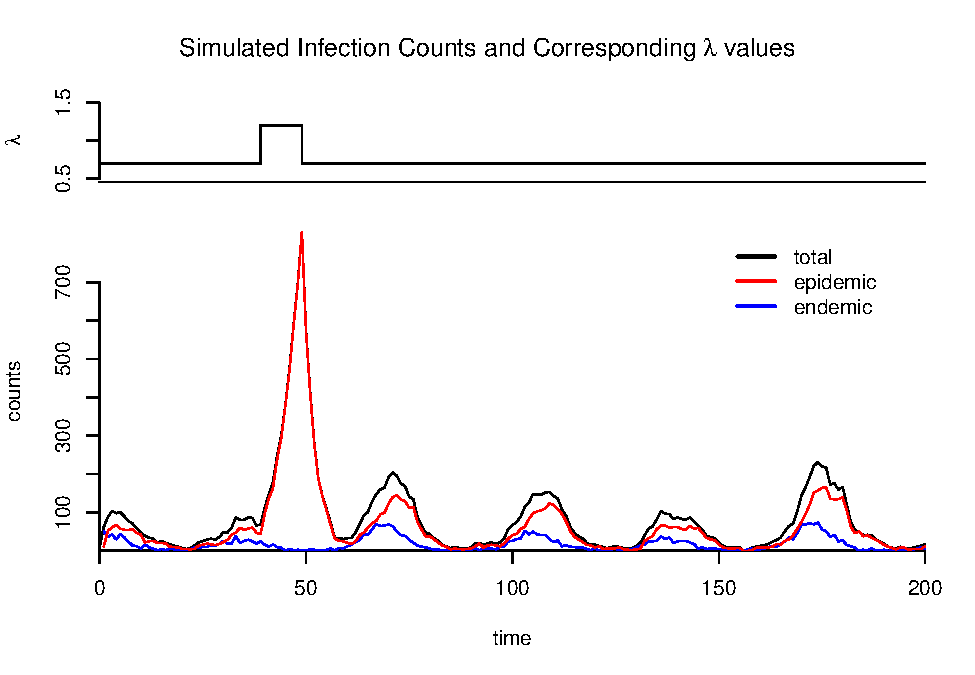
\includegraphics{thesis_draft_files/figure-latex/simulation figure-1.pdf}
\caption{\label{fig:figs}plotting example}
\end{figure}

\hypertarget{model}{%
\section{Model}\label{model}}

\hypertarget{likelihood}{%
\subsection{Likelihood}\label{likelihood}}

\[P(Z|Z_0) = \prod_{t=1}^b P(Z_t|Z_t{-1})\] Where

\[Z_t|Z_{t-1} \sim Pois(\nu_t + \lambda_tZ_{t-1})\]

\[\log{\nu_t} = \gamma_0 +  \gamma_{1}\sin(\rho l t)+\gamma_{2}\cos(\rho l t)\]

\[ \lambda_t =  \begin{cases} \lambda^{(1)} & t < \theta_0 \\
\lambda^{(k)}, & \theta_{k} \leq t < \theta_{(k-1)} \\
\lambda^{(K+1)}, & t \geq \theta_K \end{cases}\]

\hypertarget{priors}{%
\subsection{Priors}\label{priors}}

The prior values for the \(\gamma\) parameters are normally distributed
with a large variance to describe a large uncertainty.

\[\gamma_i \sim N(0, 3I_3), i \in \{0,1,2\}\]

Since the \(\lambda\) values parameterize a Poisson distribution, the
prior is set to be Gamma distributed, it's conjugate prior.

\[ \lambda^{(k)} \sim Gamma(1, 1),\ k \in \{1, \dots, K + 1\} \] The 1,
1 parameterization represents a vague prior.

A Uniform prior distribution is set on the number of changepoints. That
is

\[P(K = k) = 1/N\] and the probability of a specfic location for a
change point given the number of changepoints is unformly distributed
among all the possible changepoints

\[P(K = k) \sim 1/n,\ k \in \{1,\dots,n\}\]
\[P(\theta|K=k) = \binom{N}{k}^{-1}\]

Then the unnormallized posterior is

\[ P(Z_t|Z_{t-1},\theta, K, \lambda^{(1)}, \dots, \lambda^{(K+1)}, \gamma_0, \gamma_1, \gamma_2)*P(\theta|K)*P(K)*P(\prod_{k=1}^{k+1}\lambda^{(k)} )*P(\prod_{i=0}^2 \gamma_i)  \]

\hypertarget{graph-data}{%
\section{Graph Data}\label{graph-data}}

We would now like to extend our data from a univariate time series of
counts \(Z_t\) to a multiple time series of counts \(Z_{i,t}\) where
\(i\) now indexes separate time series. In this case, \(i\) indexes
individual cities where \(Z_i\) represents the infectious disease counts
in city \(i\).

We then model a contact network between each of these cities modeled as
an Erdos-Renyi random graph \(G\). That is we define a vertex set
\(\{1, \dots, N_v\}\) corresponding to each city \(i\) and time series
\(Z_i\) and for unique \(i, j \in V\) represent an undirected edge
between any two cities. The probability of an edge existing exists with
probability \(p\). Then for a particular graph \(G \in G\), if
\(\{i,j\} \in G\) we say \(e_{i,j} = 1\) and \(0\) otherwise. Now we
have

\[X_{it}: \text{infected count in city } i \text{ at time step } t \text{, due to endemic factors}   \]
\[Y_{it} : \text{infected count in city } i \text{ at time step } t \text{, due to epidemic factors}   \]

\[Z_{i,t+1} = X_{i,t} + Y_{i,t}: \text{infected count in city } i \text{ at time step } t \]
As before we have the epidemic component as
\(X_{i,t} \sim Pois(\nu_t)\). For the epidemic component we now have

\[Y_{i,t}|G \sim ~ Pois\big(\lambda_t*\sum_{j\neq i}^{N_v}Z_{j,t}*1[e_{i,j}=1]+ \lambda_tZ_{i,t} | G\big) \]
\[G|p \sim ER(N_v, p)\] so the probability of
\(G|p = \prod_{i \neq j} p^{1[e_{i,j}=1]}(1-p)^{1-1[e_{i,j}=1]}\) and if
\(p\sim U(0,1)\) then each graph is equally likely with probability
\(1/\binom{N_v}{2}\).

That is the epidemic component for city \(i\) is the sum of all counts
in every city \(j\) connected to \(i\) in addition to the counts in city
\(i\).

\hypertarget{migration}{%
\subsection{Migration}\label{migration}}

One issue with this model is that connecting two cities double the
infectivity parameter and also have similar counts, which is a strong
assumption that likely is not seen in real data. Further it would not
realisitically capture the situation where there is a single large
infectious in one city and multiple small infectious surrounding it. To
handle this, a migration parameter \(m\) is introduced.

\hypertarget{bayesian-inference}{%
\section{Bayesian Inference}\label{bayesian-inference}}

In Bayesian analysis, we aimt to calculate the posterior distribution of
the parameters given the data via Bayes' theorem.

\[ P(\text{parameters}|\text{data}) = \frac{P(\text{data}|\text{parameters})P(\text{parameters})}{P(\text{data})} \]

One issue is the computation of \(P(\text{data})\) which is given by
\(\int P(\text{data}|\text{parameters})P(\text{parameters})\) over the
entire parameter space. With many parameters this integral it typically
analytically intractable. To deal with this issue ({\textbf{???}})
writes many of the distributions as conjugate priors etc (tk elaborate)
and uses Markov Chain Monte-Carlo (MCMC) methods for some.

In this work we primarily appeal to MCMC methods.

\hypertarget{markov-chain-monte-carlo}{%
\subsection{Markov chain Monte-Carlo}\label{markov-chain-monte-carlo}}

(tk terrible explanation)

A Markov Chain is a sequence of random variables \((X_n)\) where
\(P(X_n)\) depends only on \(X_{n-1}\).

A probability distribution on the states of a Markov Chain is said to be
a stationary distribution \(\pi\) i

That is a distribution \(\pi\) is a stationary distribution of the
Markov Chain with transition probabilities \(P\) if

\[ \pi = \pi P \]

In Markov chain Monte Carlo (MCMC), the algorithm generates samples from
a given posterior dist \(\pi\) by constructing a Markov chain with
stationary distribution \(\pi\)

One method for constructing the chain is the Metropolis-Hastings
Algorithm

\hypertarget{metropolis-hastings-aglorithm}{%
\subsection{Metropolis-Hastings
Aglorithm}\label{metropolis-hastings-aglorithm}}

We start with a Markov Chain with proposal distribution \(q(i,j)\).

We then modify \(q\) in the following way to obtain a Markov Chain with
stationary distribution \(\pi\).

\begin{enumerate}
\def\labelenumi{\arabic{enumi}.}
\tightlist
\item
  From the current state \(X_n = i\) propose a new state \(j\) according
  to \(q\).
\item
  Compute the acceptance probability
\end{enumerate}

\[a(i,j) = \min{\big(\frac{\pi(j)q(j,i)}{\pi(i)q(i,j)},1\big) }\]

\begin{enumerate}
\def\labelenumi{\arabic{enumi}.}
\setcounter{enumi}{2}
\tightlist
\item
  Generate \(U \sim Unif(0,1)\)
\item
  If \(U < a_{ij}\) then accept the move and \(X_n = j\) otherwise
  reject and \(X_n = i\).
\end{enumerate}

This new Markov Chain has a transition probability

\[p(i,j) = q(i,j)a(i,j)\]

Assuming \(a(i,j) < 1\)

\[ \begin{aligned} \int \pi(i)*p(i,j) & = \int\pi(j)*p(j,i) \\
\int \pi(i)q(i,j)\frac{\pi(j)q(j,i)}{\pi(i)q(i,j)} & = \int\pi(j)*q(j,i)*a(j,i) \\ \int \pi(j)*q(j,i)*1 & = \int\pi(j)*q(j,i)*a(j,i)
\end{aligned}\]

\hypertarget{mcmc-implementation}{%
\section{MCMC/ Implementation}\label{mcmc-implementation}}

Here I describe the Metropolis Hastings algorithms used to generate
samples from the two-component disease model (gamma, lambda, theta) and
the underlying graph.

\ldots{}

\hypertarget{change_gamma-change_lambda}{%
\subsection{change\_gamma,
change\_lambda}\label{change_gamma-change_lambda}}

The gamma and lambda parameters are updated in blocks via a standard
Metropolis-Hastings step. The gamma and lambda proposals are each drawn
from Multivariate Normal (MVN) distributions centered as the current
parameter values. That is the proposed parameter vectors \(\gamma^*\)
and \(\lambda^*\) are drawn from \(MVN(\gamma, \sigma_\gamma I_3)\) and
\(MVN(\lambda, \sigma_\lambda I_{K+1})\) where \(I_n\) is the identity
matrix of dimension \(n\). The variance of the distributions is scaled
as \(\sigma_\gamma\) and \(\sigma_\lambda\) which are hand selected to
improve mixing.

Since the Normal distribution is symmetric, the Hastings ratio is 1 so
the acceptance ratio is the ratio of the log-likelihoods between the
current and proposed steps.

One potential issue is that gamma and lambda are used to compute the
parameter of a Poisson distribution, but the Normal distribution
proposals could potentially propose invalid parameter values. To remedy
this, the proposal operator checks to see whether the proposed parameter
value is valid (in this case positive) and automatically rejects the
proposed state (staying in the current state). This can lead to
inefficient mixing as a step is ``wasted''. This inefficiency can be
resolved by using a non-symmetric proposal distribution such as
log-normal or a truncated normal and an adjustment of the Hastings ratio
to compensate for the asymmetry. However this does not seem to be an
issue in the simulated cases.

\hypertarget{change_theta}{%
\subsection{change\_theta}\label{change_theta}}

This operator proposes a new location for one of the current change
points \(\theta_1,\dots, \theta_K\). A change point,
\(\theta_k, k \in \{1, \dots, K\}\) is selected uniformly at random from
all current change points. Then the proposed location \(\theta_k^*\) is
selected from values between
\(\{\theta_{k-1}+1,\dots, \theta_{k+1}-1\}\) uniformly at random. For
\(\theta_1\) and \(\theta_k\) the proposed values are from
\(\{0,\dots, \theta_1-1\}\) and \(\{\theta_K+1,\dots, N\}\)
respectively.

The \(\lambda\) are then updated to match the newly proposed location
as:

\[ \lambda_t =  \begin{cases} \lambda^{(1)} & t < \theta_0 \\
\lambda^{(k^*)}, & \theta_{k^*} \leq t < \theta_{(k^*-1)} \\
\lambda^{(K+1)}, & t \geq \theta_K \end{cases}\]

Since the proposal is generated uniformly at random between
\(\theta_{k-1}\) and \(\theta_{k+1}\), contribution to the Hastings
ratio is 1. Furthermore since the \(\lambda\) values are
deterministically generated from current \(\lambda_k\) values and the
\(\theta_k^*\) values, the overall Hastings ratio is 1 and the
acceptance rate is the ratio of the likelihoods.

\hypertarget{birthdeath_theta-reversible-jump-mcmc}{%
\subsection{birth/death\_theta reversible jump
mcmc}\label{birthdeath_theta-reversible-jump-mcmc}}

To handle the dimension jumping of the model (between different number
of changepoints) we use Reversible Jump MCMC.

Since the model can jump between a collection of possible models
\(\{M_k, k \in \{0,1,\cdots,n-1\}\}\) where \(k\) indexes the number of
possible changepoints.

The issue comes from the fact that we can only compare points in the
parameter space if they're defined on the same probability space.

To properly do so we need to use a Reversible Jump MCMC as implemented
in ({\textbf{???}}).

For a birth step a new changepoint is chosen uniformly at random from
all possible timesteps that aren't currently changepoints. To perform
the Reversible Jump algorithm we procede as follows:

\begin{enumerate}
\def\labelenumi{\arabic{enumi}.}
\tightlist
\item
  Draw \(u \sim Unif(0,1)\)
\item
  The following proposals for the new \(\lambda\) values are from
\end{enumerate}

\[\lambda*(\frac{u}{1-u})^{(\theta_1-\theta_0)/(\theta_2-\theta_0)}\]
\[\lambda*(\frac{1-u}{u})^{(\theta_2-\theta_1)/(\theta_2-\theta_0)}\]

That is the new \(\lambda\) values are a compromise between the original
value as a function of where the new changepoint is factored in.

\begin{enumerate}
\def\labelenumi{\arabic{enumi}.}
\setcounter{enumi}{2}
\tightlist
\item
  Acceptance probability; In order to determine the acceptance
  probability for the proposal, the corresponding death move must also
  be determined. In death move a current changepoint is selected
  uniformly at random and then removed. Then the \(\lambda\) values are
  changed deterministically such that if the newly proposed changepoint
  is removed (and the heights were the same as newly proposed ones),
  then the new height should be the original height.
\end{enumerate}

Then the new proposal ratio would be

\[ \frac{P(death)}{P(birth)}\frac{P_{death}(\theta^*\rightarrow\theta)}{P_{birth}(\theta\rightarrow \theta^*)*P(u)} = 1*\frac{\frac{1}{K+1}}{\frac{1}{N-K}} = \frac{N-K}{K+1} \]
The \(P(birth)\) and \(P(death)\) are the probabilities of proposing a
birth or death step and are selected such that \(P(birth) = P(death)\).
The probability of being in the proposed state \(\theta^*\) and
returning to \(\theta\) is the probability of selecting the newly added
changepoint \(\theta_{k^*}\) and deleting it. This occurs with
probability \(1/K+1\) since the changepoints are selected uniformly at
random and there are \(K+1\) changepoints in the proposed state.
Similarly the probability of the current proposal state is \(1/N-K\)
since there are \(N-K\) possible timesteps to add. Since
\(u \sim U(0,1)\) then \(P(u) = 1\) and the reverse move is
deterministic so it's probability is also 1.

Finally the Jacobian is given by

\[ |J_{birth}| = (\lambda_1 + \lambda_2)^2/\lambda_0\] For the death
proposal we have

\[ \frac{P(birth)}{P(death)}\frac{P_{birth}(\theta^*\rightarrow\theta)}{P_{death}(\theta\rightarrow \theta^*)*P(u)} = 1*\frac{\frac{1}{N-(K-1)}}{\frac{1}{K}} = \frac{K}{N-(K-1)} \]
And the Jacobian is
\[|J_{death}| = 1/|J_{birth}| = \lambda_0/(\lambda_1 + \lambda_2)^2\]

\hypertarget{graph-proposals}{%
\section{Graph Proposals}\label{graph-proposals}}

The proposed graph is stored as an adjacency list. To create make
proposals in the graph space the follow operators are used.

\hypertarget{flip_edge}{%
\subsection{flip\_edge}\label{flip_edge}}

Flip edge randomly samples an edge by randomly sampling two vertices at
random without replacement. If the edge is currently is the adjacency
list then it is removed, if it is not in the adjaceny list then it is
added. Since reversing a flip is equivalent to flipping that edge again,
the Hastings ratio is 1.

This proposal does not appear to mix well and this maybe due to the fact
that when the graph is sparse then the probabilty of adding an edge is
higher than deleting an edge and vice versa.

\hypertarget{add-and-delete}{%
\subsection{add and delete}\label{add-and-delete}}

The add edge operator samples uniformly at random from all edges in
\(G\\G\) that is all edges not currently in the graph and then adds it
to the graph. The delete edge operator randomly samples from all edges
currently in graph and removes it.

The Hastings ratio then becomes

\[ \frac{\frac{1}{edges + 1}}{\frac{1}{N_E - E}} = \frac{N_E-E}{edges + 1} \]
and the Hastings ratio for removing an edge is given by

\[ \frac{\frac{1}{N - (E - 1)}}{\frac{1}{ E}} = \frac{edges}{N_E-(E-1)} \]

\hypertarget{degree-preserving-swap}{%
\subsection{Degree Preserving Swap}\label{degree-preserving-swap}}

The degree preserving swap was implemented to allow changes to the graph
structure while maintaining the degree of connectivity of each vertex.
This was implemented by selecting two edges (v11, v12) and (v21, v22)
and attempting to form the edges (v11, v22) and (v12, v21). If both
edges are not already in the graph then the swap is made. If either or
both edges exists, then the proposed swap is rejected. Since the
proposed swap is reversed by randomly selecting (v11, v22) and (v12,
v21), the Hastings ratio is 1 and the acceptance ratio is the ratio of
the likelihoods.

\hypertarget{rewire}{%
\subsection{Rewire}\label{rewire}}

Rewire randomly selects an edge (v1, v2) and deletes it from the
adjacency list. It then randomly samples a vertex v3 and forms the edge
(v2, v3). Since the reverse move is selecting the edge (v2, v3) and then
rewiring (v1, v2), the Hastings ratio is 1

\hypertarget{results}{%
\section{Results}\label{results}}

\hypertarget{two-component-model-on-simulated-data}{%
\subsection{Two-Component Model on Simulated
Data}\label{two-component-model-on-simulated-data}}

\hypertarget{graph-estimation-on-fixed-two-component-model}{%
\subsection{Graph Estimation on Fixed Two-Component
Model}\label{graph-estimation-on-fixed-two-component-model}}

\hypertarget{conclusiondiscussion}{%
\section{Conclusion/Discussion}\label{conclusiondiscussion}}

\hypertarget{citations}{%
\section*{Citations}\label{citations}}
\addcontentsline{toc}{section}{Citations}

\hypertarget{refs}{}
\leavevmode\hypertarget{ref-held_two-component_2006}{}%
Held, Leonhard, Mathias Hofmann, Michael Höhle, and Volker Schmid. 2006.
``A Two-Component Model for Counts of Infectious Diseases.''
\emph{Biostatistics} 7 (3): 422--37.
\url{https://doi.org/10.1093/biostatistics/kxj016}.


\end{document}
